\documentclass[pdftex,12pt]{article}
\usepackage{mysty}
\begin{document}

\maketitlepage

\setcounter{tocdepth}{3}

\section*{Executive Summary}
\label{sec:exec}

The rise of the American biofuel industry will initiate social,
political, and environmental advancements, such as decreased
dependency on foreign oil, mitigation of pollutants, and slowed
climate change. The Obama administration's \textit{Growing America's
  Fuels} plan hopes to produce 36 billion gallons of biofuels annually
before 2022 and is limiting the use of currently popular corn
feedstocks to just 15 billion gallons per year. The remaining 21
billion gallons per year must come from new, advanced feedstocks.

\begin{figure}[h!]
  \centering
  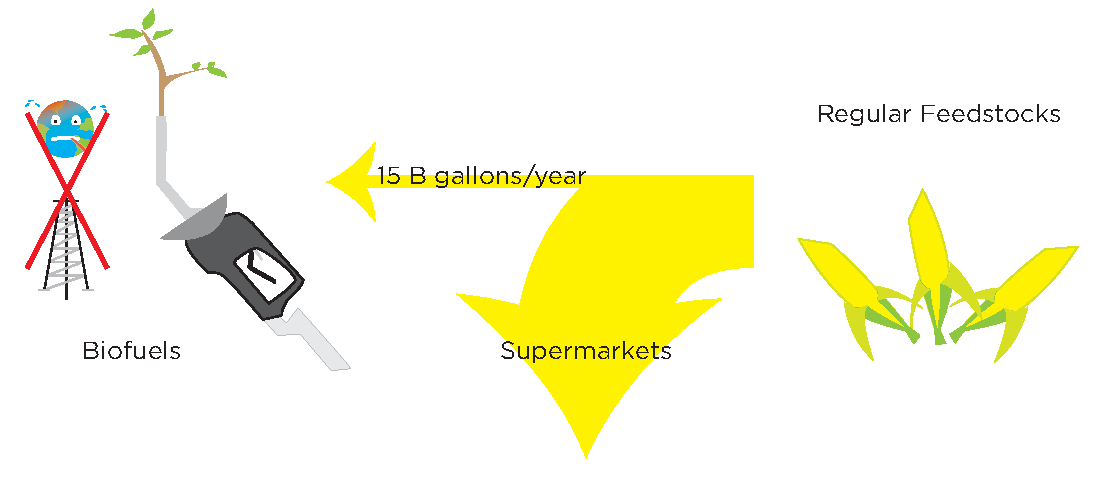
\includegraphics[width=\linewidth]{img/cornaintenough}
\end{figure}

In laboratory results, algae outshines all other feedstocks, having
the highest useable energy concentration and therefore the most
efficient land usage. As a monoculture, it can be optimized through
species selection and bioengineering leading to even greater land
efficiency. Sora hopes to build algae farms to take advantage of
algae's potential. Sora's novel bioreactor design effectively uses
control afforded by closed systems to increase the effective light
penetration depth and maximize growth efficiency. The growth
efficiency can be further enhanced by obtaining \co\ to feed the algae
from factories and power plants, sequestering carbon emissions as a
byproduct.

\begin{figure}[h!]
  \centering
  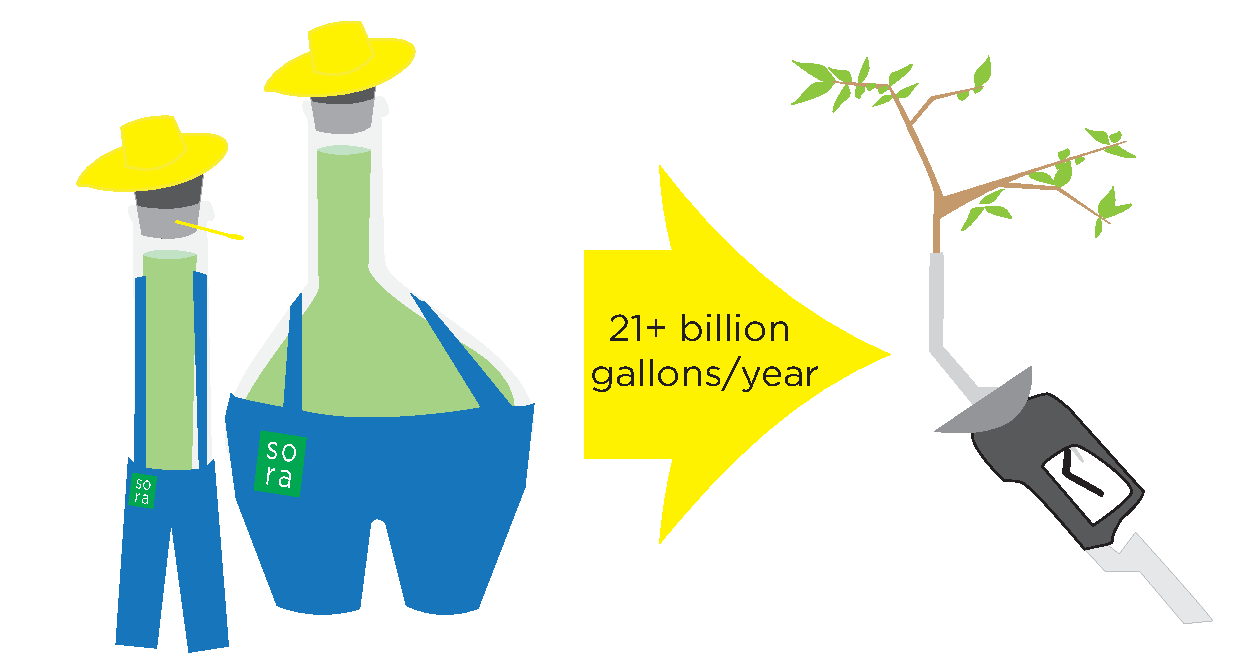
\includegraphics[width=\linewidth]{img/algaebrosalgaefarms}
\end{figure}

\begin{wrapfigure}{r}{0.31\textwidth}
  \begin{center}
    \vspace{-20pt}
    
\includegraphics[width=0.3\textwidth]{img/cut}
    \vspace{-20pt}
  \end{center}
\end{wrapfigure}

Today, there exist only a few algae farms. However most suffer from
two main issues: a lack of scalability and inefficient open-pond
designs. The rest are run by biofuel companies, which split their
efforts between growing algae and optimizing fuel processing. Sora's
aim is to specialize in algae growth and work with these companies in
order to achieve comparative advantage, accelerating the hopes of the
the political vision. Sora's competitors thus become its major market,
supplying their exponential demand for algae biomass. Even the current
day consumption of algae is considerable --- several lucrative
industries such as pharmaceuticals and nutritional supplements use
mass quantities --- and Sora hopes to provide for today and the
future.

Sora's initial steps involve lab and pre-pilot phases to demonstrate
and hone its design while producing salable biomass. The pilot and
demonstration phases will follow as larger iterations, including newly
learned lessons, and will demonstrate the baked-in scalability of the
design. From these, we hope to attract further customers and strategic
partners. Appreciating the difficulty of expanding in a capital
intense industry, the target date for commercialization is 2015, in
time to meet the 2022 deadline for increased biofuel
production. Current financial analysis indicates that the break-even
point and the ensuing profits will occur after the fifth year of
commercial operation.

\begin{figure}[h!]
  \centering
  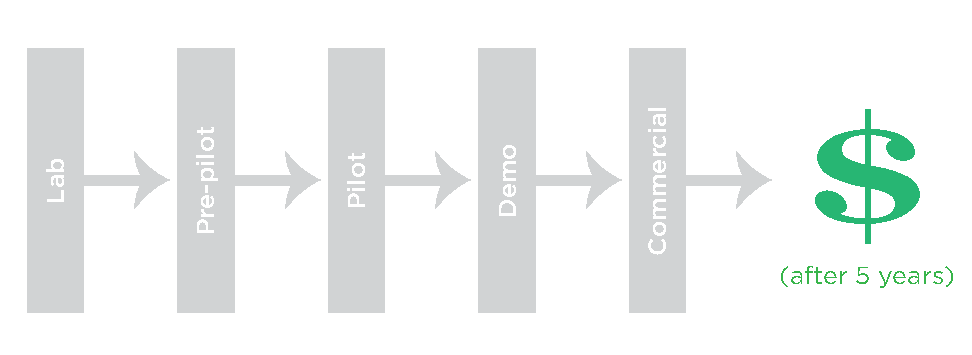
\includegraphics[width=\linewidth]{img/steps}
\end{figure}

Biofuels, particularly those derived from algae, provide the solution
to many of today's problems. Such green fuels help the environment
systematically, consuming waste carbon and staving off global climate
change, and even reducing harmful drilling operations. This new
industry will also create enormous opportunities for employment and
will decrease foreign oil dependency. By striving to help society
and clean up the world, Sora hopes to provide a valuable service and
by using efficient technology, will make it profitable.

\newpage

\tableofcontents
\newpage

\section{Products and Services}
\label{sec:products_services}

\subsection*{Product}

\subsubsection*{Description and Function}
\label{product:description}

Sora's product is a system designed to generate pure algae biomass on
a large scale and for a low price. The product also has the capacity
to sequester moderate amounts of \co\ from any \co\ source. The system
is composed of two major subsystems: the algae growth region and the
stream processing units. The stream processing is similar to many
other industrial processes and is responsible for managing the heat,
oxygen, and \co\ levels in the algae streams. The growth region uses a
patent pending tubular bioreactor system to maximize effective depth
and provide a sealed, supportive environment for the algae. These
technologies together form a bioreactor which maximizes land
efficiency while remaining cheaper than alternative closed bioreactor
designs.

\begin{comment}
  The algae growth region consists of a lattice of interwoven,
  transparent polymer tubes exposed to sunlight and containing an
  algae and water solution flowing through the tubes. There are many
  possible variations of the weave that could be implemented, based on
  the conditions of the sequestration site and including factors such
  as terrain slope and sunlight intensity. For instance, several tubes
  might be twisted or braided together, then further woven into a
  textile composed of the tubes.

  The algae solution flowing through the growth region passes through
  the stream processing units at regular intervals. These processing
  units are responsible for introduction and dissolution of nutrients
  and \co\ into the algae solution, for solution cooling, and for
  removal of oxygen and a small portion of the solution itself. Though
  it is possible that these elements may be incorporated into a single
  tower, the design of the stream processing unit currently consists
  of several components in series.

  Carbon dioxide will be dissolved into the algae solution using
  countercurrent flow, with flue gases bubbling upwards and water
  flowing downwards, allowing for the most complete transfer of the
  gases. Dissolved oxygen within the algae solution, beyond a certain
  limit, will inhibit the uptake of \co\ by the algae. Excess
  dissolved oxygen will be removed from the solution using sparging, a
  technique in which a gas passed through a liquid may be used to pull
  another gas out of solution. The portion of the algae solution that
  is harvested will be refined using a combination of flocculation,
  filtration, and pressing to obtain a more concentrated algae
  product.
\end{comment}

\subsubsection*{Key Features and Needs Satisfied}
\label{product:features}
As the biofuels industry continues to expand, there will be an ever
increasing demand for cheap and pure algae biomass. Currently, those
in the process of commercializing biofuels are more focused on the
process of extracting usable hydrocarbons from algae than on producing
cheap, pure algae on a large scale. As a result, current biofuels
projects are increasingly unable to economically scale their algal
production while maintaining purity to meet the needs of their growing
biofuels extraction processes. In this market, Sora's product fulfills
the need for an ever growing demand for large volumes of pure, cheap
algae biomass. Additionally, the pure cheap algae produced also serves
to satisfy the needs of other consumers of algae biomass, such as the
pharmaceutical, food, cosmetic, and fertilizer industries.

In addition to providing a large stock of algae biomass, the product
also has the capacity to sink large volumes of \co. Thus, the product
also offers heavy carbon dioxide polluters an effective, reliable, and
sustainable method to sequester their \co output.

\subsubsection*{Advantage of the Product}
\label{product:advantage}

While there exist many algae biomass producers, few are focused solely
on the large scale production of algae biomass. Essentially all
producers are also vested in the biofuels extraction process, and are
thus forced to split resources between algae production and biofuels
extraction. Sora, by focusing solely on the large scale production of
pure algae biomass, is well equipped to out-compete those forced to
split their resources.

\paragraph{Compared to Other Closed Bioreactor Systems}
\label{product:compare_closedloop}

Increasingly, those in the field of large scale algae biomass
production are looking to closed systems. Sora's edge in this regard
lies in the utilization of a novel tubing system which requires far
less external structural support than any other existing large scale
closed-loop algae bioreactors. This product is also designed to take
better advantage of the light incident upon a given area of land by
increasing the effective penetration depth. This feature is achieved
again through the physical layout. The combination of better land use
and cheaper support infrastructure impart a key advantage to Sora's
algal biomass production system over other closed loop systems.

\paragraph{Compared to Open Pond Systems}
\label{product:compare_openpond}

An alternative to closed loop systems are the open pond systems, an
older technology, in which algae is grown in ponds exposed to open
air. One of the benefits of Sora's system over open pond systems is
the additional control exerted over the flow of water. By passing the
algae solution through Sora's bioreactor system, it is possible to
control the average exposure of algae to light, as well as the
frequency through which algae pass through a light-dark cycle. Open
pond systems are only able to approximate this through controlled
mixing, leaving many parameters undefined and difficult to
quantify. Additionally, the closed system protects against
contamination from other algal species, while open pond systems are
open to invasive algal species competing with the desired algae,
resulting in lower growth efficiencies. The combination of various
elements targeted at improving the system's efficiencies over other
systems, including open ponds, will allow for the optimization of the
most important metric: bioproductivity per dollar.

\paragraph{Compared to Geologic Carbon Capture and Storage (\CCS)}
\label{product:compare_underground}

Lastly, in the realm of carbon sequestration, there currently exist
few alternatives, notably, Geologic \CCS. Sora's product provides a far
more sustainable method for carbon sequestration over geologic
\CCS. Geologic \CCS\ is a process in which carbon dioxide is separated
from flue gases, liquefied, then pumped underground. A key liability
in \CCS is that it would be crucial to monitor the injected sites for
several hundred years, given that a \co leak would be catastrophic,
both on a local and global level. 

\subsubsection*{IP Protection}
\label{product:ip}

The team is in the process of developing a patent for the U.S. Patent
and Trademark Office (\textsc{uspto}). The Georgia Tech Office of
Technology and Licensing (\textsc{otl}) will perform a prior art
search and patentability assessment on the patent work completed and
will work to finalize and submit the patent application. In addition
to the U.S. patent application, the team plans on filing a placeholder
with the international community through the Patent Cooperation Treaty
(\textsc{pct}) which will allow for filing international patents
within 30 months.

\section{Market Analysis}
\label{sec:market}

\subsection{Primary Market: Biofuel Suppliers}
\label{sec:primary-market}

Currently, 12 billion gallons of biofuels are produced for domestic
consumption annually. The majority of these biofuels are generated via
transesterification processes on corn oils; however, the governmental
goal for 2022 demands production of 36 billion gallons per year with a
limit of only 15 billion of year produced from corn feedstocks. This
goal has recently been readdressed and expanded by President Obama's
\textit{Growing America’s Fuel} program with additional organization
and funding as directed by the EPA and the USDA's Research, Economics,
and Education (REE) and Forest Service (FS) departments.

This policy is indicative of the growing movement towards domestic,
sustainable, and carbon-neutral fuel sources. Societal and political
pressures are making biofuels increasingly desirable and many
companies (see Appendix E) are testing laboratory methods for biofuel
creation from various biomass sources, with a special focus on
algae. This is unsurprising as compared to other investigated biofuel
feedstocks, algae has a number of distinct advantages. It is resilient
to environmental changes, can be grown very quickly under ideal
nutrient conditions, is being targeted by advanced genetics research
to improve strains, and is one of the most carbon-negative feedstocks
available.

With these planned expansions in biofuel production and consumption of
feedstock, there is a great deal of room for the kind of large scale
algae farm Sora's technology supports. In order to produce the additional
21 billion gallons of biodiesel annually that must come from non-corn
feedstocks, biofuel producers would require an annual supply of 140
million tonnes of algae, or the yearly output of 86 full-scale Sora
installations.

\subsection{Other Algae Consumers}
\label{sec:other-algae-consumers}

The biofuel market may be today's most promising consumer of algae,
however algae biomass is valuable in many other markets as well. In
particular, there is interest in using algae biomass in the food,
pharmaceutical, cosmetic, and fertilizer markets. Though these
customers are not expected to represent a large percentage of the
market, some of their needs may develop much more quickly than the
biofuels market thus acting as support capital during Sora's
development.

\subsection{Socio-Environmental Impact}
\label{sec:socio-envir-impact}

As mentioned, algae is a more carbon-negative feedstock (according to
the National Renewable Energy Laboratory, algae is 250 to 750 times
more efficient in land usage than corn) than most other proposed
biofuel feedstocks and faces little competition with food markets
unlike corn. Already this provides a strong societal and environmental
impetus for expanding algae growth. As a second factor, Sora's algae
growth bioreactors are designed to carefully control the algae's
growth environment and plug into nutrient sources as needed. This
design allows for direct linkage of Sora's algae farms to heavy carbon
producers such as industrial manufacturing plants or coal-fired power
plants.

In particular, the US emits over 1950 million metric tons of \co\
every year and that number is expected to grow by 16.8\% over the next
20 years. Though current carbon trade markets do not value this carbon
very highly, it is very possible that new policy on carbon cap and
trade will change that. In either case, Sora's algae farms could
recycle these carbon emissions directly benefiting power plants by
disposing of excess \co\ and benefiting Sora by providing a cheap
source of needed \co.

Today over 580 coal-fired power plants exist and it is unreasonable to
expect these plants to disappear any time soon. Thus it is also
unreasonable to believe the environmental damage they are causing will
be simply mitigated by new sources of power. Instead, Sora believes
that the algae bioreactors can help to ease this transition.

\section{Competition}
\label{sec:competition}

\subsection*{Existing Competition}
\label{competition:existing}

There are many companies with technologies and business models that
pose some form of competition to Sora. Most generally, businesses
which produce biofuel feedstocks will be the main competitors. These
competitors are divided into two main subgroups: companies producing
ethanol and biodiesel from corn and soybeans, and the burgeoning
number of new startups centered around algae-based biofuels.

The first type of competition is corn and soybean-based biofuel
producers. The market for ethanol has grown tremendously over the past
five years. This is due in large part to major government subsidies
and an ethanol mandate in the Energy Policy Act of 2005 requiring that
gasoline sold in the U.S. must contain an increasing amounts of
ethanol in coming years.

Feedstocks such as corn and soybeans have been the simplest to employ
to meet the ethanol mandate since the farmland and infrastructure to
grow these crops is readily available. However, these crops are
plagued by two main problems which put algae at an advantage. First,
producing these fuels from corn and soybeans is energy inefficient;
indeed, more energy is required to produce the ethanol than the energy
contained in the fuel. Second, both crops require vast tracts of land
to produce sizable amounts of fuel as compared to algae.  In
particular, corn and soybeans produce 18 gallons and 50 gallons per
acre per year, respectively, while algae can produce 5,000-15,000
gallons per acre per year.

The second subgroup of competitors are startup companies that are in
the algae growing business. Although there are now over twenty
startups in the algae producing field, none have yet moved from the
lab or pilot phase to a full-scale commercial operation. A list of
algae-related startups and their proposed markets are shown in Table
\ref{tab:competitors} in the Attachments.

The primary driver behind most of these startup companies is to
produce biofuels - ethanol and/or biodiesel - from algae. Most
companies are attempting to both grow the algae and process it into
biofuels. This business model differs from corn and soybean-based
ethanol, where the crop production is segmented from the fuel
processing.

In contrast to these algae startups, Sora's business model focuses
solely on growing algae and does not encompass biofuel processing. In
this way, Sora will produce a feedstock of algae to sell to companies
with the technology and expertise to process it into biofuels in much
the same way that farmers across the Midwestern U.S. grow and provide
corn and soybeans to ethanol refineries.

Besides the business model, the other main difference that sets Sora
apart from other algae startups is the technology. The current
competitive field can be split into companies which use open pond
systems and those which use closed bioreactors to grow algae. While
many companies use open ponds, those using closed bioreactor systems
(see Table \ref{tab:competitors} in the Attachments) experience
boosts in efficiency and control in excess of the additional material
and construction costs required for closed bioreactors.

Sora's bioreactor has clear advantages over open systems in its
ability to maximize land efficiency and prevent external
contamination. There is a technological edge over other closed
bioreactors in that this system is designed to use cheap, natural
sunlight and to maximize the light efficiency of the algae growth
process. This design will result in lower material cost, higher land
efficiency, and more scalable installations than other closed
bioreactor systems.

\subsection*{Future Competitors}
\label{competition:future}

The future competitive landscape may include other forms of renewable
energy in addition to biofuels. This will be contingent on the market
success of electric vehicles. Currently, the overwhelming market for
biofuels, such as those that will be produced from algae, is in
transportation. If major technological advances are made in electric
vehicle technology which make them economically competitive with
traditional, hydrocarbon fuel burning vehicles, renewable energy
technologies, such as wind and solar, will be in much greater demand
to produce the electricity needed to power a growing fleet of electric
vehicles.

If electric vehicles do increase significantly in overall market
share, there will be less of a demand for biofuels for
transportation. However, if this trend does occur, the algae-based
biofuel market is expected to evolve and continue to flourish, perhaps
shifting to being used for electricity production alongside other
renewables.


\section{Marketing and Sales}
\label{sec:marketing}

\subsection*{Target Customers}
\label{marketing:target}
Sora's target customers fall within two categories due to Sora's two
pronged approach to generating revenue streams. The first category of
customers includes companies which own and operate coal-fired power
plants. These companies are currently under pressure to reduce their
carbon emissions. Sora's product provides a means by which these
companies can strategically improve their financial and legal position
by mitigating the regulatory and financial risks associated with their
carbon emissions. In comparison to other carbon sequestration
technologies, Sora's product offers greater land efficiency and a
continuous harvest cycle. The second category of customers includes
companies which produce biofuels. Biofuels are generated from biomass
sources, with corn feedstock currently in the lead as the most used
biomass. However, algae is a much more sustainable feedstock due to
its relatively high land usage efficiency. The Obama administration
has set as a goal the production of 36 billion gallons of biofuels
annually by 2022, though only 15 billion gallons may be derived from
corn, due to the inefficiency of corn. In order for biofuel companies
to produce the remaining 21 billion gallons, they must be supplied
with approximately 140 million tonnes of algae biomass
annually. Sora's product can fill this need, using the combination of
high concentrations of \co\ derived from the first category of
customers and its novel bioreactor design.

\subsection*{Distribution System}
\label{marketing:distribution}

Sora's team plans to implement the product by making use of
pre-existing plant infrastructures and subcontractors already tailored
to power plant feed and waste processing. This cooperation is
necessary due to the capital intensive nature of the product and the
need to adapt to various scales and implementation details of each
plant. Fortunately, Sora's solution can fit this niche well as many
components are already popular in industrial processing and novel
components can be easily constructed.

\begin{comment}
\subsection*{Pricing Policy}
\label{marketing:pricing}
THIS WAS TERRIBLE
\end{comment}

\subsection*{Marketing \& Sales Plan}
\label{marketing:plan}
Sora's team plans on selling the product at the commercial scale by
first developing a strong working relationship with power plant
customers, initiated by touring their facilities and exhibiting to
them the demonstration plant as a proof-of-concept. The team will then
work directly with these customers on a case-by-case basis to
establish how they can best adopt the product to their specific power
plant. A strong contact with our power plant customer base will aid
the successful adoption of Sora's product, and as such, the Sora team has
already initiated contact with various power producers in the
Southeast. Additionally, Sora's team will simultaneously be developing
a customer base among biofuel producers. Development of contracts for
the supply of algae biomass early in the game would strongly benefit
such biofuel producers, as they would be guaranteed a feedstock supply
at a low cost.

In the first year of commercial operation, Sora plans on developing
two independent installations situated near different power plants,
and another three installations in the second year. Following this, no
installations will be developed until the break-even point is achieved
after five years of commercial operation. This break-even point
accounts for the costs of the pre-pilot, pilot, and demonstration
plants. The profit generated in the seventh year will then be
reinvested into the construction of more installations and into
research and development.

\section{Operations and Manufacturing}
\label{operations}

\begin{comment}
\subsection*{Operations and Manufacturing Strategy}
\label{operations:strategy}
The production of the full algae farm system will be distributed
between the various subsystems. The primary subsystems are growth
regions, nutrient mixing chambers, water coolers, \co\ diffusion
systems, and algae harvesting and drying systems. The growth regions,
comprised of a network of clear polymer tubes, will be provided by an
external manufacturer and cut to our specifications.

\end{comment}

\subsection*{The Operations and Manufacturing Process}
\label{operations:process}
A firm versed in large-scale construction projects and familiar with
projects involving the transport of fluids will be responsible for
supervision of the construction. This company's responsibilities will
include facilitation of the construction process and oversight of the
integration of the various subsystems at each location.

The specifics of the manufacturing process require detailed discussion
of the technology. These details are given in a patent application
currently being processed by the U.S. Patent and Trademark Office and
thus will not presently be divulged.

\begin{comment}
  The bioreactor growth tubes can be made of a material transparent to
  visible sunlight, such as silicone, vinyl, or clear PVC. The growth
  tubes will be purchased wholesale from a major distributor and
  delivered to the bioreactor site. On site, the tubes will first be
  braided together into long strands.  The number of tubes in each
  strand, and the length of each strand, will be dictated by
  geographic conditions at the bioreactor site. For example, if the
  average solar flux intensity at the site is relatively high, more
  tubes will be braided together in order to distribute the light to
  the algae most effectively. Alternatively, if the solar flux is
  relatively low, fewer tubes will be braided together in order to
  maximize the amount of light within each tube. The length of each
  strand will be determined based on the geography and topography of
  the bioreactor site. Following the tube braiding, the strands will
  be woven into a 2-dimensional matrix. The particular variety of
  weaving pattern will again be dependent on geographic conditions at
  the bioreactor site, in particular the average solar flux
  intensity. The size of the matrix will be dependent on the land
  available at the site.

  Nutrient mixing will be accomplished in a mixing chamber located
  adjacent to one or more areas of growth tubes, depending on the size
  of the bioreactor site. These mixing chambers will contain the
  nutrients to be supplied to the algae in concentrated form.  Each
  nutrient mixing chamber will be fitted with automated hopper systems
  which control the rate of nutrient injection into the growth tubes.
  Additionally, a mixer system will be in place to increase the rate
  at which the nutrients dissolve. The components necessary for
  nutrient mixing, namely the hoppers and the driving mechanism, will
  be obtained through suppliers in those industries.

  The water cooling system will utilize any one of a number of
  different types of industrial scale water chillers commercially
  available from wholesale manufacturers. Similar to the nutrient
  mixing chamber, the water cooling system will be located in a
  centralized location with direct access to one or more adjacent
  sections of growth tubes. The water from each of section of growth
  tubes will be piped into the cooling system to extract the heat
  generated by solar infrared absorption and from excess heat
  introduced by the \co\ gases.

  The algae harvesting and drying system will be installed in a
  central location with respect to several sections of woven growth
  tubes. This system will consist of several components, each of which
  will be purchased from a wholesale distributor. First, an algae
  collection chamber will be constructed to hold a large quantity of
  algae-laden water. The algae collection chamber may be outfitted
  with nozzles to inject a commercially available flocculant, such as
  Prestol, into the algae solution to aggregate and concentrate the
  algae solution in the bottom of the chamber. Alternatively, the
  chamber may be fitted with an outlet through a ceramic micro-flow
  filter to concentrate the algae solution into a separate, smaller
  chamber. Downstream from the chamber any one of several commercially
  available drum presses will be installed to dry the concentrated
  algae solution for shipment. As with the other subsystems, the
  integration will be supervised by the managing construction firm.

  Though the piping for the liquids and the ductwork for the gases
  will be sourced separately from independent suppliers, integration
  of the overall system will be completed by the managing construction
  firm after the materials are delivered to the site. The pumps and
  the forced draft fan, used to facilitate the transfer of fluids,
  will be obtained and incorporated in a similar manner.
\end{comment}

\subsection*{Key Suppliers and Subcontractors}
\label{operations:suppliers}
One of the key processes involved in the creation of the sequestration
system is the integration of the various subsystems. This process will
require the services of a construction firm familiar with the concerns
involved in construction of emission control systems at coal-fired
power plants. This firm will be chosen for its combination of
expertise in engineering, construction, fabrication, and project
management. Additionally, this firm should have an existing customer
base within the power industry and have worked on emissions mitigation
systems with power providers in the past. Potential firms under future
review include Alberici Enterprises, Lauren Engineers and
Constructors, Kiewit Energy, and Bechtel Power.

Certain components of the carbon sequestration system, such as the
hopper, mixer, piping, ductwork, fans, and pumps will be obtained from
the appropriate commercial suppliers. The choice of suppliers will
ultimately be determined by the location of the power plant site on a
case-by-case basis, allowing for minimization of transportation costs
and other potential cost-related benefits to working with the local
supply chain.

\begin{comment}
  \subsection*{Financial Characteristics}
  \label{operations:financial}
  Sora's financial outlook in its first year (June 2010 - June 2011)
  can be separated into three main types of expenses: 1) pre-pilot
  construction costs, 2) pre-pilot operating costs, and 3) business
  operation expenses. We aim to begin construction of a pre-pilot
  system of our algae-based sequestration system within the coming
  year. The pre-pilot will be our first major step on the road to a
  full-size, commercial scale sequestration system.  Its purpose will
  be to prove the concept of our technology, to optimize the energy
  and space efficiency of the technology, and to attract potential
  investors and customers for a pilot operation. The projected cost
  for the materials to construct the pre-pilot are given in Tables
  \ref{tab:costs1} and \ref{tab:costs2} in the Attachments, and totals
  approximately \$30,000.

  The second main expense type for Sora's first year will be the
  operating costs for the pre-pilot.  These expenses include
  utilities, such as power and water, along with necessary nutrients
  to support the operation of the pre-pilot. The projected cost for
  these items is given in Table \ref{tab:costs3} in the Attachments
  and totals approximately \$30,000.

  The final expense type is Sora's business-related expenses. These
  expenses include office needs, marketing, insurance, legal fees, and
  intellectual property protection.  The projected cost for each of
  these is given in Table \ref{tab:costs4} in the Attachments and
  totals approximately \$450,000.
\end{comment}

\subsection*{Research and Development}
\label{operations:research}

With the goal of improving biomass production efficiency, several
areas will be focused on for further research and development. The key
criterion is bioproductivity per dollar, where the financial concerns
involve all parts of the system life cycle. Simply put, this may be
accomplished by either increasing the amount of algae produced per
unit of the system or by driving down the cost of the system.

Algal production is fundamentally limited by losses involved in
photosynthesis. However, alternating light-and-dark cycles have been
shown to increase bioproductivity. This cycle is induced in Sora's design
by the physical layout, but the cycle frequency may be varied by using
different flow rates or tube arrangements. However, increased flow
rates may induce too great of a shear for certain strains of
algae. These effects will be studied and the results incorporated into
later designs.

Several methods of driving down the system cost have been proposed. At
large installations, material costs may significantly drop if cheaper
alternative materials which still meet the team's specifications are
found. Also, operation costs may be decreased by better recycling
water or heat energy. Methods and apparatuses with which to improve
efficiency in utilities may be found commercially and will be studied
for their ability to be integrated into our system.

\subsection*{Future Products and Services}
\label{operations:future}

As demand for algae grows, larger installations of the Sora system
will be desirable.  In order to accommodate demand, Sora intends to
create strategic partnerships with other industries. Much as power
plants benefit from supplying the system with \co\, waste water
treatment may benefit from feeding into the system. Waste water
includes many nutrients helpful in growing algae, serving to offset
nutrient costs while decreasing the load on the treatment
facilities. Also, further means of introducing \co\ into the system
will be offered. For example, researchers at the Georgia Institute of
Technology have identified a means of capturing carbon from car
exhaust.  This technology may be mated to Sora's system, serving to help
recycle the carbon.

\section{Finances}
\label{sec:finances}

The financial analysis, a crucial element in determining Sora's
financial viability, required the accurate cost estimation of various
factors. A detailed analysis was carried out for the pre-pilot plant
(see Appendix A), in addition to general analyses for the construction
and operation of a commercial installation, and a break-even analysis.

The operation of an installation requires several inputs and outputs,
dictating the expenditures and revenues. The sequestration of \co\ and
the sale of algae biomass both represent revenue streams, while the
use of electricity, water, nutrients, and operational labor represent
expenditures. The expenditures were estimated using known current
values. The estimated total annual expenditure amounted to \$32.8
million. The cost for sequestration of \co\ was drawn from the current
cost in the European carbon markets, while the cost of algae biomass
was based on a combination of current prices of crude oil and the
current prices of comparable biodiesel feedstocks. The combination of
cash inflows generates an estimated annual revenue of \$52.2
million. This operation cost breakdown may be viewed in Appendix B.

The construction of the installation is a capital expense and includes
equipment as well as labor costs. The break down of this expense may
be seen in Appendix C. It was estimated that the capital expense of a
single installation will be \$86 million.

The break-even analysis, shown in Appendix D, took the full life of the company into consideration. The pre-pilot, pilot, and demonstration phase costs were all included in expenditures. Revenue streams were only generated
after the commercial stage was reached. The break-even point, the
point at which the lifetime revenue negated the lifetime expenditures,
occurred after five years of commercial operation, or after eight
years of overall operation.

\section{Management}
\label{sec:management}

\subsection*{Corporate Structure}
\label{management:structure}

Sora Corporation was legally incorporated in October 2009 as a General 
Corporation in the state of Delaware. Sora's office in the State of 
Delaware is 160 Greentree Drive, Suite 101, County of Kent, Dover, 
Delaware 19904. Sora's registered agent at this address is National
Registered Agents, Inc. Sora's address for its operations in Atlanta, GA
is 5390 Cottage Farm Road, Alpharetta, GA 30022.

Sora's corporate structure is made up of its Board of Directors and Officers. 
Directors may convene meetings of Sora's stockholders. Currently, each
of the five founders and the advisors given below serve on the Board of
Directors. The Board of Directors is also responsible for choosing the 
Officers of Sora Corporation. Each of the five founders is currently an 
Officer with their respective positions given below.
 
\subsection*{Founding Entrepreneurial Team}
\label{management:founders}
 
\subsubsection*{Will Boyd, \textit{President}}
 
Will is a 4th year Physics and Computer Science major at the Georgia
Institute of Technology. Will's interest in founding Sora comes from
his interest in renewable energy technologies and business strategies to 
employ them in the marketplace. Will has been actively involved in 
undergraduate research in physics and computing both at Georgia Tech and
at the \textsc{atlas} experiment at the European Organization for Nuclear
Research (\textsc{cern}) in Geneva, Switzerland.
 
\subsubsection*{Andrew Punnoose, \textit{Vice President of Research \& Development}}
 
Andrew is a 4th year Aerospace Engineering student at the Georgia
Institute of Technology. He is currently an undergraduate researcher
in the Intelligent Controls System Lab (\textsc{ICSL}) Lab, working on
the design of a flapping wing micro aerial vehicle
(\textsc{MAV}). Andrew's interest in founding Sora was a result of his
fascination with biological systems and his interest in renewable
energy.
 
\subsubsection*{Sanjay Challa, \textit{Vice President of Business Development}}
 
Sanjay is a 4th year Biomedical Engineering major at Georgia
Tech. Sanjay worked at National Instruments (NI) as an Engineering
Leadership Program Intern, where he built a medical device from
scratch on the technical marketing team, and set an industry standard 
in \textsc{iso} and \textsc{fda} compliance documentation for the use 
of NI's products in creating medical devices. Sanjay is also the Curriculum 
Chair on the Biomedical Engineering Student Advisory Board, where he 
serves as a liaison between students and faculty.
 
\subsubsection*{Joseph Abrahamson, \textit{Vice President of Marketing \& Sales}}
 
Joseph is a 4th year Biomedical Engineering major at Georgia
Tech. Joseph has made advanced studies in mathematics and chemistry
while practicing poignant graphic design and working in
neuroengineering labs in his downtime. Joe has always been interested
in developing alternative energy technologies and thus eagerly took 
up the chance to start Sora.
 
\subsubsection*{Kento Masuyama, \textit{Vice President of Finance}}
 
Kento is a 4th year Aerospace Engineering student at the Georgia
Institute of Technology. He was a member of the 1st place team in the
2007 \textsc{aiaa} Undergraduate Team Space Transportation System
Competition, and he currently works in the Space Systems Design
Laboratory at Georgia Tech. His interest in this project stems from a
fascination of and love for nature, as well as the prospect of
overcoming an important challenge.
 
\subsection*{Future Management Roles}
\label{management:future}
 
In the future, the team plans to add additional positions to the
management and technical teams as they become necessary. In
particular, it will be advantageous to hire a “Go-to-Market”
\textsc{ceo} as the endeavor progress from pre-pilot to pilot
phase. For this position, the plan is to recruit an individual with
extensive experience in the chemical processing industry and in
planning and building pilot and/or demo stage plants. In addition, a
\textsc{cfo} and \textsc{cto} may be added in the transition from the
pilot phase to demo phase. Sora will fill both of these roles with
individuals with experience building technology-oriented start-up
companies, though the \textsc{cto} role may be filled by one of the
founding members.
 
\subsection*{Board of Advisors}
\label{management:advisors}
 
\subsubsection*{L. Franklin Bost, \textit{\footnotesize MBA, ISDA}}
 
Mr. Bost is currently Director of Design Instruction at the Wallace
H. Coulter Department of Biomedical Engineering, Georgia Institute of
Technology and Emory University. Mr. Bost has over 35 years of business 
experience in strategic planning, new product development, senior 
management and leadership with companies in medical, consumer and 
industrial markets. He is President and Chief Executive Officer of 
SpherIngenics, Inc. and early-stage biotechnology company specializing
in stem cell delivery technologies. He was previously president of 
Porex Surgical Inc. which developed, manufactured and marketed 
implantable products for craniofacial reconstruction.

Mr. Bost holds an \textsc{mba} from the University of North Carolina and a
Bachelor of Product Design degree from North Carolina State University. He 
is a member of the Industrial Designers Society of America (\textsc{idsa}),
Society of Biomaterials, Biomedical Engineering Society, and the American 
Association for the Advancement of Science.
 
\subsubsection*{Ben Hill, \textit{\footnotesize MBA}}
 
Ben Hill is currently Senior Business Advisor of VentureLab, a
product development and commercialization group for early stage
ventures at Georgia Tech. As a member of VentureLab, Ben focuses on
clean technology research and commercialization. In addition, Ben is
an adjunct professor in the Georgia Tech College of Management. Prior
to joining VentureLab, Ben was the co-founder of Cirronet, Inc., a
wireless products company that was later acquired by RF Monolithics. 
Ben has been an invaluable member of the Board of Advisors since Sora's 
inception. Ben holds an \textsc{mba} from Emory University and a Master's 
of Arts in Religion from Yale University.

\subsection*{Awards}
\label{sec:awards}

In February 2009, the founders won second place in the “Ideas to
Serve” (\textsc{I2S}) Competition sponsored by the College of
Management at Georgia Tech for early stage venture products. The
awards from I2S competition included recognition at the Business Plan
Competition awards ceremony and a \$500 cash prize.

In March 2009 the founding entrepreneurial team won the InVenture
Prize, a competition focused on fostering innovation and
entrepreneurship at Georgia Tech. The prize for winning the
competition included a \$10,000 cash prize, free patent filing through
the Georgia Tech \textsc{OTL}, and connections with various firms
affiliated with the Georgia Tech community.
 
\section{Future Growth}
\label{sec:growth}

\subsection*{Positive Contingencies}
\label{growth:positive_contigencies}
There are two major contingencies that could provide a major boost to
the market for carbon sequestration in the near future. Current
climate legislation moving through Congress, such as the Waxman-Markey
bill and the Kerry-Boxer bill, would be a major positive contingency
for the business model, as it would attach a significant cost to
carbon dioxide emissions. Such a cost would drive a change in the
operations of a variety of industries through the basic principles of
economics. Climate legislation will most likely come in the form of a
cap and trade system. This would be a major asset to Sora business as
carbon emissions do not presently pose a financial burden to emitters
(although such industries can already reduce their emissions and sell
carbon credits to help recoup the costs incurred).
 
A second major positive contingency would be the passage and/or
renewal of substantial subsidies for biofuel production. Indeed,
recent U.S. legislation requires vast increases each year in ethanol
production and its use as an additive in gasoline. This legislation
has established ethanol as a permanent commodity and instilled
confidence in biofuel startup ventures. Sora's business model places
it in a position to benefit from these and other federal, state, or
local policies that benefit biofuel producers. Government incentives
for biofuels would in effect increase the market potential for algae
as feedstock for biofuels, making this product more profitable for
coal-burning power plants.

\subsection*{Areas for Future Growth \& Development}
\label{growth:areas}
There are a number of avenues for growth that will be explored as
Sora develops in the next five years. The first of these is
international intellectual property protection. At present, the
U.S. is behind the curve on clean energy and climate legislation
compared to many other developed nations, including those in the EU
and Japan. As a result of this discrepancy, carbon credits are
currently worth significantly more in those countries than in the
United States. As such, it could prove quite beneficial to Sora
business to file patents in one or more of these countries to have
access to more lucrative carbon markets overseas. A second area for
further growth is other \co\ producing industries, including natural
gas and petroleum-burning power plants, oil refineries, paper mills,
and concrete factories.

\section{Exit Strategy}
\label{sec:exit}
Sora is a long-term vision and a project that the owners hope will continue
to benefit society past their own involvement. It is the intention of
the owners to see through the first several years after
commercialization to the point where the balance is positive and the
company can be sold for substantial profit. At that point, the owners
intend to sell their shares first to other members of the founding
team and eventually to willing external entities.

In the case that the proposed plan does not meet the owners' criteria
for success, all necessary measures will be taken to minimize losses
to the owners and investors. All resources and equipment will be sold
to help cover outstanding debts, and interest will be assessed for
external parties to license the intellectual property. The criteria
for success will be discussed with all interested stakeholders and are
subject to review at each phase in the development of Sora. Through
the demo phase, success will be monitored monthly, and past
commercialization, quarterly. 

The owners have done a break-even analysis and expect a positive
balance after five years of commercial operation. The same analysis
has allowed for a projection of acceptable losses throughout this
period; significant excess of this value will result in the process of
closing the endeavor and recouping losses.

\newpage

\section{Appendices}
\label{sec:attachments}


\begin{figure}[h]
  \footnotesize
  \centering
  \begin{tabularx}{,95\textwidth}{l}
    \textbf{\large Cash Flow Analysis}
  \end{tabularx}
  \begin{tabularx}{,45\textwidth}{ll}
    \textbf{Cash Inflows} & \\
    \toprule
    Algae sales & \$50,000,000 \\
    \co\ sequestration & \$2,200,000 \\
    \\
    \\
    \\
    \\
    \hline    
    \textbf{Total} & \$52,200,000 \\
    \bottomrule
  \end{tabularx}
  \begin{tabularx}{,45\textwidth}{ll}
    \textbf{Cash Outflows (Expenses)} & \\
    \toprule
    Nutrients                   & \$2,900,000     \\
    Electricity                 & \$9,600,000     \\
    Water                       & \$1,000,000     \\
    Insurance                   & \$10,000,000    \\
    Payroll                     & \$5,000,000     \\
    Capital purchases           & \$4,300,000 \\
    \hline    
    \textbf{Total} & \$28,500,000 \\
    \bottomrule
  \end{tabularx}\\[3em]

  \begin{tabularx}{,9\textwidth}{Xr}
    \textbf{Summary} & \\
    \toprule
    Inflow & \$52,200,000 \\
    Expenses & \textcolor{red}{\$28,500,000} \\
    Other Outflow & \textcolor{red}{\$4,300,000} \\
    \hline    
    \textbf{Total} & \$19,400,000 \\
    \bottomrule
  \end{tabularx}
\end{figure}

\newpage

\begin{sidewaystable}[H]
  \footnotesize
  \centering
  \begin{tabularx}{,85\textwidth}{lXXXlllll}
    \multicolumn{9}{l}{\textbf{\large Break Even Analysis}} \\
    \toprule
    \textbf{Year} &    \textbf{Phase} & \textbf{Number Built} & \textbf{Total Installations} & \textbf{Installation Cost} & \textbf{Operations Cost} & \textbf{Cash in} & \textbf{Yearly Total}  & \textbf{Balance} \\
    \hline
    2011   & Prepilot &    --- &        0 & \$3,185,195   & \$1,214,815   & 0             & \textcolor{red}{\$4,400,010}   & \textcolor{red}{\$4,400,010}   \\
    2012   &    Pilot &    --- &        0 & \$9,555,586   & \$3,644,444   & 0             & \textcolor{red}{\$13,200,031}  & \textcolor{red}{\$17,600,041}  \\
    2013   &     Demo &    --- &        0 & \$28,666,759  & \$10,933,333  & 0             & \textcolor{red}{\$39,600,092}  & \textcolor{red}{\$57,200,133}  \\
    2014   &        1 &      2 &        2 & \$172,000,554 & \$65,600,000  & \$104,400,000 & \textcolor{red}{\$133,200,554} & \textcolor{red}{\$190,400,687} \\
    2015   &        2 &      3 &        5 & \$258,000,831 & \$164,000,000 & \$261,000,000 & \textcolor{red}{\$161,000,831} & \textcolor{red}{\$351,401,518} \\
    2016   &        3 &      0 &        5 & 0             & \$164,000,000 & \$261,000,000 & \$97,000,000   & \textcolor{red}{\$254,401,518} \\
    2017   &        4 &      0 &        5 & 0             & \$164,000,000 & \$261,000,000 & \$97,000,000   & \textcolor{red}{\$157,401,518} \\
    2018   &        5 &      0 &        5 & 0             & \$164,000,000 & \$261,000,000 & \$97,000,000   & \textcolor{red}{\$60,401,518}  \\
    2019   &        6 &      0 &        5 & 0             & \$164,000,000 & \$261,000,000 & \$97,000,000   & \textbf{\$36,598,482}   \\
    2020   &        7 &      2 &        7 & \$172,000,554 & \$229,600,000 & \$365,400,000 & \textcolor{red}{\$36,200,554}  & \$397,928      \\
    2021   &        8 &      2 &        9 & \$172,000,554 & \$295,200,000 & \$469,800,000 & \$2,599,446    & \$2,997,374    \\
    2022   &        9 &      2 &       11 & \$172,000,554 & \$360,800,000 & \$574,200,000 & \$41,399,446   & \$44,396,820   \\
    \bottomrule
  \end{tabularx}
\end{sidewaystable}

\newpage

 \begin{sidewaystable}[H]
  \footnotesize
  \centering
  \begin{tabular*}{\textwidth}{p{5cm} p{4cm} p{5cm} p{2cm} p{2cm} p{2cm}}
    \multicolumn{6}{l}{\textbf{\large Pre-pilot Expense Breakdown}} \\
    \toprule
    \textbf{Item}     & \textbf{Supplier}    & \textbf{Note}     & \textbf{Qty}    & \textbf{Cost/Item}    & \textbf{Total Cost} \\
    \hline
    \\
    \multicolumn{6}{c}{\textbf{Bioreactor}}\\ 
    \hline
    \\
    Silicone tubing  & Ryan Herco Flow Solutions & Support pre-pilot & 300 ft & \$1.2/ft & \$600 \\
    Low shear water pumps   & Watson Marlow & Support pre-pilot & 2 & \$150 & \$300 \\
    \\
    \multicolumn{6}{c}{\textbf{CO$_2$ Dissolution System}}\\ 
    \hline
    \\
    Bubble breaking mesh    & Woven Wire    & Support pre-pilot    & 1    & \$60    & \$60 \\
    CO$_2$ hose    & Marine Depot    & Support pre-pilot    & 100 ft.    & \$0.99/ft    & \$100 \\
    CO$_2$ regulator    & Marine Depot    & Support pre-pilot    & 1    & \$150    & \$150 \\
    CO$_2$ tanks    & Cylinder Mart    & Support pre-pilot    & 2    & \$115    & \$230 \\
    Dissolution tank    & Cal Aqua Labs & Support pre-pilot & 1 & \$105 & \$105 \\
   Water pump    & Grainger    & Support pre-pilot    & 4    & \$106    & \$424 \\
    \\
    \multicolumn{6}{c}{\textbf{Control System}}\\ 
    \hline
    \\
    Backup hard drive    & Western digital    & Support pre-pilot    & 1    & \$250    & \$250 \\
    Cables    & Various    & Support pre-pilot    & N/A    & \$500    & \$500 \\
    Computer    &   Various    & To support pre-pilot    & 1    & \$500    & \$500 \\
    DAQ BNQ    & National Instruments    & Support pre-pilot    & 1    & \$2,000 & \$2,000 \\
    DAQ board    & National Instruments    & Support pre-pilot    & 1    & \$800    & \$800 \\
    Flow sensors    & RCM Industries    & Support pre-pilot    & 5    & \$120    & \$600 \\
    Light sensors    & Macam Photometrics Ltd.    & Support pre-pilot    & 4    & \$30    & \$120 \\
    Power supply    & Sola HD    & Support pre-pilot    & 1    & \$1,000    & \$1,000 \\
    \\
    \multicolumn{6}{c}{\textbf{Lab Supplies}}\\ 
    \hline
    \\
    Balance    & Mettler Toledo    & Algae productivity analysis       & 1    & \$2,200    & \$2,200 \\
    Cell counter    & Beckman Coulter    & Algae productivity analysis     & 1    & \$10,000    & \$10,000 \\
    Cuvette Rack    & International Crystal    & Store algae samples               & 1    & \$45     & \$45 \\
    Glassware    & Indigo Instruments    & Beakers, burets, pipets        & 1    & \$200    & \$200 \\
    Lab tables    & Hertz Furniture Systems    & Support lab equipment    & 2    & \$225    & \$450 \\
    Optical Cuvettes    & International Crystal    & Transport algae samples         & 1    & \$850    & \$850 \\
    Optical microscope    & Edmund Scientific & Algae productivity analysis & 1 & \$120 & \$120 \\
    UV-vis Spectrophotometer    & Hewlett-Packard    & Characterize algae samples    & 1     & \$8,000    & \$8,000 \\
    \bottomrule
  \end{tabular*}
    \caption{Pre-Pilot Construction Costs}
    \label{tab:costs1}
    \end{sidewaystable}

\begin{sidewaystable}[H]
  \footnotesize
  \centering
  \begin{tabular*}{\textwidth}{p{5cm} p{4cm} p{5cm} p{2cm} p{2cm} p{2cm}}
    \multicolumn{6}{l}{\textbf{\large Pre-pilot Expense Breakdown}} \\
    \toprule
    \textbf{Item}     & \textbf{Supplier}    & \textbf{Note}     & \textbf{Qty}    & \textbf{Cost/Item}    & \textbf{Total Cost} \\
    \hline
    \\
    \multicolumn{6}{c}{\textbf{Nutrient Mixing System}}\\ 
    \hline
    \\
    Automated valve    & Clippard Instrument Laboratory  & Support pre-pilot    & 2    & \$50    & \$100 \\
    Dry chemical mixing tank & TrashCanDepot    & Support pre-pilot    & 1 & \$200 & \$200 \\
    Water pump    & Grainger    & Support pre-pilot    & 2    & \$106    & \$212 \\
    Water filter    & General Electric & Support pre-pilot & 4 & \$11 & \$44 \\
    \\
    \multicolumn{6}{c}{\textbf{Shipping Fees}}\\ 
    \hline
    \\
    \\
    \multicolumn{6}{c}{\textbf{Tools}}\\ 
    \hline
    \\
    Circular saw    & Amazon    & Construct/maintain pre-pilot    & 1    & \$160    & \$160 \\
    Clamps    & Amazon    & Construct/maintain pre-pilot    & N/A    & \$105    & \$105 \\
    Cordless drill    & Amazon    & Construct/maintain pre-pilot    & 1    & \$350    & \$350 \\
    Drill bits    & Amazon    & Construct/maintain pre-pilot    & N/A    & \$150    & \$150 \\
    Electric sander    & Amazon    & Construct/maintain pre-pilot    & 1    & \$70    & \$70 \\
    Grinder    & Amazon    & Construct/maintain pre-pilot    & 1    & \$90    & \$90 \\
    Hammers    & Amazon    & Construct/maintain pre-pilot    & N/A   & \$100    & \$100 \\
    Outdoor lighting    & Amazon    & Construct/maintain pre-pilot    & 2    & \$80    & \$160 \\
    Pipe wrenches    & Amazon    & Construct/maintain pre-pilot    & 1     & \$15    & \$15 \\
    Pliers    & Amazon    & Construct/maintain pre-pilot     & N/A    & \$35    & \$35 \\
    Power cords    & Amazon    & Construct/maintain pre-pilot    & 10    & \$35    & \$350 \\ 
    Sockets    & Amazon    & Construct/maintain pre-pilot    & N/A    & \$60    & \$60 \\
    Soldering iron    & Amazon    & Construct/maintain pre-pilot    & 1    & \$45    & \$45 \\
    Wrenches    & Amazon    & Construct/maintain pre-pilot    & N/A    & \$65    & \$65 \\
    \\
    \multicolumn{6}{c}{\textbf{Water Cooling System}}\\ 
    \hline
    \\
    Water chiller & Aqua Logic & Support pre-pilot & 3 & \$1,500 & \$4,500 \\
    \\
    \multicolumn{6}{c}{\textbf{Total Projected Pre-Pilot Construction Cost}}\\ 
    \hline
    \\
    \textbf{Total Cost} & & & & & \textbf{\$36,415} \\
    \bottomrule
    \end{tabular*}
    \caption{Pre-Pilot Construction Costs (cont.)}
    \label{tab:costs2}
    \end{sidewaystable}

\begin{sidewaystable}[H]
  \footnotesize
  \centering
  \begin{tabular*}{\textwidth}{p{5cm} p{4cm} p{5cm} p{2cm} p{2cm} p{2cm}}
    \multicolumn{5}{l}{\textbf{\large Pre-pilow Expense Breakdown}} \\
    \toprule
    \textbf{Item}     & \textbf{Supplier}    & \textbf{Note}     & \textbf{Qty}    & \textbf{Cost/Item}    & \textbf{Total Cost} \\
    \hline
    \\
    \multicolumn{6}{c}{\textbf{Nutrients}}\\ 
    \hline
    \\
    KNO$_3$ & Alfa Aesar   & Potassium Nitrate & 22.5kg/day    & \$30   & \$10,950\\
    KH$_2$PO$_4$    & Alfa Aesar    & Potassium dihydrogen phosphate    & 560kg/day & \$21   & \$7,665 \\
    MgSO$_4$ (7$\times$H$_2$O)   & Alfa Aesar    & Magnesium sulfate & 1,125kg/day   & \$26/day    & \$9,490 \\
    FeSO$_4$ (7$\times$H$_2$O)   & Alfa Aesar    & Iron(II) sulfate heptahydrate & 1.35kg/day    & \$0.06/day & \$22 \\
    H$_3$BO$_3$    & Alfa Aesar    & Boric acid    & 1.25kg/day & \$0.03/day & \$11 \\
    MnSO$_4$ (7$\times$H$_2$O)   & Alfa Aesar    & Manganese sulfate    & 1.2kg/day & \$0.03/day & \$11 \\
    ZnSO$_4$ (7$\times$H$_2$O)   & Alfa Aesar    & Zinc sulfate  & 0.1kg/day & \$0.004/day    & \$1.45 \\
    CuSO$_4$ (5$\times$H$_2$O)   & Alfa Aesar    & Copper sulfate    & 36mg/day  & \$0.0007/day   & \$0.25 \\
    Na$_2$MoO$_4$   & Alfa Aesar    & Sodium molybdate  & 10mg/day  & \$0.0008/day   & \$0.30 \\
    CO$_2$  & Pye-Barker, Fire and Safety  & Carbon dioxide & 10lb/month & \$0.85/day & \$305 \\
    \\
    \multicolumn{6}{c}{\textbf{Utilities}}\\ 
    \hline
    \\
    Power & Georgia Power & Run pre-pilot & 42,000 kWh & \$6.33/day & \$2,310 \\
    Water & City of Atlanta & Support pre-pilot & 120,000 gal & \$6.67/day & \$2,400 \\    
    \\
    \multicolumn{6}{c}{\textbf{Total Projected Pre-Pilot Operating Cost}}\\ 
    \hline
    \\
    \textbf{Total Cost} & & & & & \textbf{\$33,166} \\
    \bottomrule
    \end{tabular*}
    \caption{Pre-Pilot Operating Expenses (June 2010 - June 2011)}
    \label{tab:costs3}
    \end{sidewaystable}


\begin{sidewaystable}[H]
  \footnotesize
  \centering
  \begin{tabular*}{\textwidth}{p{5cm} p{7cm} p{5cm} p{2cm} p{2cm} p{2cm}}
    \multicolumn{5}{l}{\textbf{\large Pre-pilow Expense Breakdown}} \\
    \toprule
    \textbf{Item}   & \textbf{Note}     & \textbf{Qty}    & \textbf{Cost/Item}    & \textbf{Total Cost} \\
    \hline
    \\ 
    \multicolumn{5}{c}{\textbf{Labor}}\\ 
    \hline
    \\
    Employee salaries   & Atlanta cost of living adjusted    & 5 founders $\times$ 12 months    & \$2,000  & \$120,000 \\
    \\
    \multicolumn{5}{c}{\textbf{Conferences and Networking}}\\ 
    \hline
    \\
    Algal Biomass Summit & Registration, flights, etc. & 5 attendees & \$2,350 & \$11,750 \\
    Carbon Capture and Sequestration Summit & Registration, flights, etc. & 5 attendees & \$1,300 & \$6,500 \\
    Electric Power Conference & Registration, flights, etc. & 5 attendees & \$1,400 & \$7,000 \\
    National Algae Association Conference & Registration, flights, etc. & 5 attendees & \$1,300 & \$6,500 \\
    Power-Gen Conference & Exhibit, registration, flights, etc. & 5 attendees & \$2,600 & \$13,000 \\
    \\
    \multicolumn{5}{c}{\textbf{Insurance}}\\ 
    \hline
    \\
    Business owners policy  & Nation Wide & 5 founders & \$6,000 & \#30,000 \\
    \\
    \multicolumn{5}{c}{\textbf{Legal Expenses}}\\ 
    \hline
    \\
    Attorney fees & Contractual agreements, financing, etc & 30 hours & \$500/hour & \$15,000 \\
    Patent filings  & Australia, Brazil, Canada, China, Germany, India, Japan, Russia, South Africa, Spain, U.K.     & 11 countries    & \$25,000/country & \$275,000 \\
    \\
    \multicolumn{5}{c}{\textbf{Office Supplies}}\\ 
    \hline
    \\
    Office Supplies  &   Marketing/networking   & 5 founders  & --- & \$5,000 \\
    Internet and Phone & Marketing/networking & 1 yr & --- & \$750 \\
    Hardware and Peripherals & Productivity & 5 founders & --- & \$7,500 \\
    Office space    &   Rent and utilities    & 1   & --- & \$15,000 \\
    Software & Productivity & 5 founders & --- & \$5,000 \\
    Web domain  &   Marketing   & 1 year    & --- & \$150 \\
    \\
    \multicolumn{5}{c}{\textbf{Total Projected Cost}}\\
    \\
    \hline    \textbf{Total Cost} & & & & \textbf{\$467,450} \\
    \bottomrule
  \end{tabular*}
  \caption{Business-Related Expenses (June 2010 - June 2011)}
  \label{tab:costs4}
\end{sidewaystable}


\begin{sidewaystable}[H]
  \footnotesize
  \centering
  \begin{tabularx}{,85\textwidth}{llXXX}
    \multicolumn{4}{l}{\textbf{\large Current Competitors}} \\    
    \toprule
    \textbf{Company}                   & \textbf{Proposed Market}                                    & \textbf{Status}  & \textbf{Website}         \\
    \hline
    Algenol Biofuels                   & Ethanol production, \co sequestration                       & Pilot phase      & algenolbiofuels.com  \\
    Aquaflow Bionomic Corp             & Wastewater treatment, Biomass production                    & Pilot phase      & aquaflowgroup.com    \\
    Aquatic Energy                     & Biomass production, \co sequestration                       & Pilot phase      & aquaticenergy.com    \\
    Aurora Biofuels                    & Biodiesel production                                        & Pilot phase      & aurorabiofuels.com   \\
    Bionavitas                         & Biodiesel production, \co sequestration                     & Lab phase        & bionavitas.com       \\
    Blue Marble Energy                 & Wastewater treatment, Biomass/natural gas production        & Pilot phase      & bluemarble energy    \\
    Bodega Algae                       & Wastewater treatment, Biomass production, \co sequestration & Lab phase        & bodegaalgae.com      \\
    Carbon Capture Corp                & Biomass production, \co sequestration                       & Pilot phase      & carbcc.com           \\
    Cellana                            & Biomass production, Biofuel processing                      & Pilot phase      & cellana.com          \\
    GreenFuel Technologies Corp        & Biodiesel/ethanol production, \co sequestration             & \textit{Defunct} & greenfuelsonline.com \\
    INFINIFUEL Biodiesel               & Biodiesel production                                        & Lab phase        & infinifuel.com       \\
    Inventure Chemical Technology      & Biodiesel/ethanol production                                & Pilot phase      & inventurechem.com    \\
    Kent BioEnergy Corp                & Wastewater treatment, Biomass production, \co sequestration & Pilot phase      & kentbioenergy.com    \\
    LiveFuels                          & Biocrude production                                         & Lab phase        & livefuels.com        \\
    OriginOil Incorporated             & Biomass production, Biomass processing                      & Commercial phase & originoil.com        \\
    PetroAlgae                         & Carbon sequestration                                        & Pilot phase      & petroalgae.com       \\
    PetroSun Incorporated              & Biodiesel production                                        & Pilot phase      & petrosuninc.com      \\
    Sapphire Energy                    & Biocrude production                                         & Pilot phase      & sapphireenergy.com   \\
    Seambiotic                         & Biomass production, \co sequestration                       & Pilot phase      & seambiotic.com       \\
    Solena Group                       & Syngas production                                           & Pilot phase      & solenagroup.com      \\
    Solix Biofuels                     & Biodiesel production, \co sequestration                     & Pilot phase      & solixbiofuels.com    \\
    XL Renewables                      & Biomass production, Wastewater treatment, \co sequestration & Pilot phase      & xldairygroup.com     \\
    \bottomrule
  \end{tabularx}
  \caption{An overview of current indirect competitors.}
  \label{tab:competitors}
\end{sidewaystable}

\end{document}
